\documentclass[]{elsarticle} %review=doublespace preprint=single 5p=2 column
%%% Begin My package additions %%%%%%%%%%%%%%%%%%%
\usepackage[hyphens]{url}

  \journal{Social Science and Medicine} % Sets Journal name


\usepackage{lineno} % add
\providecommand{\tightlist}{%
  \setlength{\itemsep}{0pt}\setlength{\parskip}{0pt}}

\usepackage{graphicx}
\usepackage{booktabs} % book-quality tables
%%%%%%%%%%%%%%%% end my additions to header

\usepackage[T1]{fontenc}
\usepackage{lmodern}
\usepackage{amssymb,amsmath}
\usepackage{ifxetex,ifluatex}
\usepackage{fixltx2e} % provides \textsubscript
% use upquote if available, for straight quotes in verbatim environments
\IfFileExists{upquote.sty}{\usepackage{upquote}}{}
\ifnum 0\ifxetex 1\fi\ifluatex 1\fi=0 % if pdftex
  \usepackage[utf8]{inputenc}
\else % if luatex or xelatex
  \usepackage{fontspec}
  \ifxetex
    \usepackage{xltxtra,xunicode}
  \fi
  \defaultfontfeatures{Mapping=tex-text,Scale=MatchLowercase}
  \newcommand{\euro}{€}
\fi
% use microtype if available
\IfFileExists{microtype.sty}{\usepackage{microtype}}{}
\bibliographystyle{elsarticle-harv}
\ifxetex
  \usepackage[setpagesize=false, % page size defined by xetex
              unicode=false, % unicode breaks when used with xetex
              xetex]{hyperref}
\else
  \usepackage[unicode=true]{hyperref}
\fi
\hypersetup{breaklinks=true,
            bookmarks=true,
            pdfauthor={},
            pdftitle={Changes in accessibility to emergency and community food services during COVID-19 and implications for low income populations in Hamilton, Ontario},
            colorlinks=false,
            urlcolor=blue,
            linkcolor=magenta,
            pdfborder={0 0 0}}
\urlstyle{same}  % don't use monospace font for urls

\setcounter{secnumdepth}{0}
% Pandoc toggle for numbering sections (defaults to be off)
\setcounter{secnumdepth}{0}

% Pandoc citation processing
\newlength{\cslhangindent}
\setlength{\cslhangindent}{1.5em}
\newlength{\csllabelwidth}
\setlength{\csllabelwidth}{3em}
% for Pandoc 2.8 to 2.10.1
\newenvironment{cslreferences}%
  {}%
  {\par}
% For Pandoc 2.11+
\newenvironment{CSLReferences}[2] % #1 hanging-ident, #2 entry spacing
 {% don't indent paragraphs
  \setlength{\parindent}{0pt}
  % turn on hanging indent if param 1 is 1
  \ifodd #1 \everypar{\setlength{\hangindent}{\cslhangindent}}\ignorespaces\fi
  % set entry spacing
  \ifnum #2 > 0
  \setlength{\parskip}{#2\baselineskip}
  \fi
 }%
 {}
\usepackage{calc}
\newcommand{\CSLBlock}[1]{#1\hfill\break}
\newcommand{\CSLLeftMargin}[1]{\parbox[t]{\csllabelwidth}{#1}}
\newcommand{\CSLRightInline}[1]{\parbox[t]{\linewidth - \csllabelwidth}{#1}\break}
\newcommand{\CSLIndent}[1]{\hspace{\cslhangindent}#1}

% Pandoc header
\usepackage[table]{xcolor}
\usepackage{booktabs}
\usepackage{longtable}
\usepackage{array}
\usepackage{multirow}
\usepackage{wrapfig}
\usepackage{float}
\usepackage{colortbl}
\usepackage{pdflscape}
\usepackage{tabu}
\usepackage{threeparttable}
\usepackage{threeparttablex}
\usepackage[normalem]{ulem}
\usepackage{makecell}
\usepackage{xcolor}



\begin{document}
\begin{frontmatter}

  \title{Changes in accessibility to emergency and community food
services during COVID-19 and implications for low income populations in
Hamilton, Ontario}
    \author[Some University]{Author One}
   \ead{author1@example.com} 
    \author[Another University]{Author Two\corref{1}}
   \ead{author2@example.com} 
    \author[Some University]{Author Three}
   \ead{author3@example.com} 
    \author[Some University]{Author Four}
   \ead{author4@example.com} 
      \address[Some University]{Department, Street, City, State, Zip}
    \address[Another University]{Department, Street, City, State, Zip}
      \cortext[1]{Corresponding Author}
  
  \begin{abstract}
  In this paper we analyze the changes in accessibility to community and
  emergency food services before and during the COVID-19 pandemic in the
  City of Hamilton, Ontario. Many of these food services are the last
  line of support for households facing food insecurity; as such, their
  relevance cannot be ignored in the midst of the economic upheaval
  caused by the pandemic. Our analysis is based on the application of
  balanced floating catchment areas and concentrates on households with
  lower incomes (\textless CAD40,000, approximately the Low Income
  Cutoff Value for a city of Hamilton's size). We find that
  accessibility was low to begin with in suburban and exurban parts of
  the city; furthermore, about 14\% of locations originally available in
  Hamilton closed during the pandemic, further reducing accessibility.
  The impact of closures on the level of service of the remaining
  facilities, and on accessibility, was disproportionate, with
  system-wide losses exceeding 40\%. Those losses were geographically
  and demographically uneven. While every part of the city faced a
  reduction in accessibility, inner suburbs fared worse in terms of loss
  of accessibility. As well, children (age \(\le 18\)) appear to have
  been impacted the most.
  \end{abstract}
  
 \end{frontmatter}

\hypertarget{introduction}{%
\section{Introduction}\label{introduction}}

Food insecurity is defined as an ``inadequate or uncertain access to a
sufficient quantity and/or adequate quality of food'' due to a
household's financial limitations (Enns et al., 2020). This condition
has been associated with reductions in nutritional outcomes
(Bhattacharya et al., 2004; Kirkpatrick and Tarasuk, 2008; Olson, 1999)
and negative physical and mental health impacts in children and adults
(Elgar et al., 2021; Jones, 2017; Ramsey et al., 2011; Seligman et al.,
2010; Stuff et al., 2004). Over at least the past four decades food
banks and related services have become an essential line of defense
against food insecurity in Canadian communities (Black and Seto, 2020;
Holmes et al., 2018; Riches, 2002; Tarasuk et al., 2020). In this
respect, Canada is not unlike numerous other wealthy countries where a
systematic dismantling of the welfare state took place in the
intervening period (Tarasuk et al., 2014).

The emergence of COVID-19, the worst public health crisis since the 1918
flu pandemic, has exposed important social and economic fault lines, and
pre-existing patterns of inequality appear to have been exacerbated.
Along several other dimensions of stress (e.g., accessibility to health
care facilities, Ghorbanzadeh et al., 2021; Pereira et al., 2021a), this
seems to be the case for food insecurity as well (Laborde et al., 2020).
According to Statistics Canada (2020a), in the early stages of the
pandemic almost 15\% of individuals reported living in a household that
faced food insecurity; the risk of food insecurity was substantially
higher for households with children. The difference between households
with and without children was significant, and 11.7\% of households with
children indicated that ``food didn't last and {[}there was{]} no money
to get more'' sometimes or often, compared to 7.3\% of households
without children; likewise, 13\% of households with children indicated
that they ``{[}c{]}ouldn't afford balanced meals'' sometimes or often,
compared to 8.8\% of households without children. Additionally, Men and
Tarasuk (2021) report that about 25\% of individuals who experienced job
insecurity (a relatively common occurrence during the pandemic) also
experienced food insecurity associated with COVID-related disruptions to
employment, financial hardship, and use of food charity.

The impacts of food insecurity during the pandemic are alarming, since
diet-related diseases, such as obesity, heart-disease, and diabetes,
were already critical public health concerns in Canada prior to COVID-19
(Boucher et al., 2017). While emergency food services are not
necessarily a stable solution to food insecurity and in fact may
encourage a retrenchment of neoliberal policy (Wakefield et al., 2013),
in reality provide a resource of last instance to households in
precarious situations (Bazerghi et al., 2016). As a mid-size city
grappling with deindustrialization, Hamilton exhibits high rates of
poverty and use of emergency food services. As recently as 2019, the
Hamilton Hunger Report (HFS, 2019) noted that food banks in the city
recorded the highest number of visitors in the past 29 years; a rate of
increase greater than population growth. Most troubling, approximately
40\% of all visitors were children.

It is known that urban food environments, within which people make their
daily food choices, are essential in influencing eating behaviours and
health outcomes, based on factors such as food availability, ease of
geographic accessibility and socio-demographic variations (Paez et al.,
2010; Vanderlee and L'Abbé, 2017; Widener, 2018). However, while there
is a wealth of literature that has examined the topic of geographic
accessibility to healthy food through the ``food desert'' concept, there
has been little research into accessibility to emergency and community
food services. Previous work has explored differences in
\emph{accessing} food banks, such as how some households utilize food
banks over short periods of time while others regularly utilize food
banks as longer-term resource (e.g., Enns et al., 2020). In addition,
transportation and locational considerations have been raised as key
issues in food bank accessibility in previous qualitative research
(Smith-Carrier et al., 2017). However, we are not aware of any research
that has focused on estimating or capturing this geographic component of
accessibility.

The study of place-based geographic accessibility is concerned with
capturing the potential to reach destinations of value using the
transportation network (Páez et al., 2012). Indeed, the Government of
Canada's recent Food Policy (Agriculture and Canada, 2019) has made
``access'' to healthy food a priority for Canadian communities and
previous research suggests that such accessibility plays a key role in
user satisfaction with food bank service delivery (Holmes et al., 2018).
However, as with research into the prevalence of food deserts,
accessibility to food banks is unlikely to be evenly distributed, and
variation throughout a city can be expected due to transportation
network characteristics and the spatial distribution of service
locations and the population they are meant to serve. Furthermore,
policy responses to the COVID-19 pandemic likely have added to the
distress of vulnerable households. Non-pharmaceutical interventions
during the pandemic involving restrictions in mobility have increased
the friction of travel, in particular by transit on which low income
populations are more reliant (e.g., DeWeese et al., 2020). At the same
time, the pandemic has created additional stress for the operators of
food banks through disruptions in the supply chain (e.g., McKay et al.,
2021) as well as concerns surrounding the delivery of service in safe
conditions and possible cancellation of food service programs.

For this study, we aim to look at how the landscape of emergency food
and related services (e.g.~low-cost or free meal service providers)
available in Hamilton, Ontario, changed during the pandemic. Did the
number of open services diminish? If so, what was the accessibility to
emergency and community food services before the pandemic from the
perspective of low income households, and how has it changed during the
pandemic with respect to geographic access and congestion at remaining
sites? And finally, who are most likely to have been impacted by changes
in the accessibility landscape? This paper first looks at the
distribution of emergency and community food services before and during
the pandemic. Then, we use the balanced floating catchment area approach
of Paez et al. (2019) to investigate the accessibility situation. For
this, we adopt a fully disaggregated approach based on parcel-level
data. Socio-economic and demographic data are drawn from the latest
Census of Canada (2016), whereas travel information is from the most
recent regional travel survey from 2016. This paper follows reproducible
research recommendations (see Brunsdon and Comber, 2020), and the
research was conducted using open source tools for transportation
analysis (Lovelace, 2021). The data and code needed to reproduce the
analysis are available in a public repository (see Supplemental
Material).

\hypertarget{food-insecurity-and-emergency-and-communal-food-services-in-canada}{%
\section{Food Insecurity and Emergency and Communal Food Services in
Canada}\label{food-insecurity-and-emergency-and-communal-food-services-in-canada}}

Food insecurity is the inability to acquire and consume an adequate
amount or good quality food, leading to inadequate nutrient intake
(Kirkpatrick and Tarasuk, 2008) and poorer physical and mental health
outcomes (Ramsey et al., 2011; Seligman et al., 2010; Stuff et al.,
2004). In this regard, food insecurity is a major population health
concern, particularly among Canadians at socio-economic disadvantage
(Bazerghi et al., 2016). Official government surveys such as the
Household Food Security Survey Module (HFSSM), the Canadian Community
Health Surveys (CCHS), the Longitudinal and International Study of
Adults (LISA), and official classifications determined by Health Canada
in relation to socio-demographic variables offer some insight into food
insecurity in Canada (Gundersen et al., 2018; Kirkpatrick and Tarasuk,
2008; Tarasuk and Vogt, 2009).

Nationally, analysis of the 2011-2012 CCHS has previously revealed that
food insecurity impacts approximately 12.3\% of Canadian households
(Tarasuk et al., 2014). Using the same data, Tarasuk et al. (2019) found
higher odds of food insecurity amongst households relying on social
assistance, those without a university degree or with children under the
age of 18, and individuals that lived alone, renters, and those
identifying as Aboriginal. While surveys revealed that only 20 to 30
percent of those experiencing food insecurity were found to frequent
food banks in Canada (Tarasuk et al., 2014), pre-pandemic research from
Ottawa (Enns et al., 2020) and Vancouver (Black and Seto, 2020) suggests
that long-term users tend to be older, have health or mobility
challenges, live in large households, and are less likely to have
employment income. In terms of geography, previous research conducted at
the provincial scale using data from the 2011-2012 CCHS found that the
prevalence of food insecurity ranged across the country from 11.8\% of
households in Ontario to 41\% of households in Nunavut (Tarasuk et al.,
2019).

Food banks - sometimes also referred to as `food pantries' and `food
shelves' - originated as a community response to aid those with
inadequate food by voluntarily offering them meals and ingredients
(Loopstra and Tarasuk, 2012; Riches, 2002). Although in their origin
food banks were meant to be provide a temporary solution to accommodate
those in hunger due to job retrenchments and economic downfalls since
the 1980s, over time many have evolved into a community practice to
secure food supplies for those in need (Loopstra and Tarasuk, 2012;
Wakefield et al., 2013). In Canada, the number of food banks has
steadily increased in the past few decades (Wakefield et al., 2013). The
largest database of food banks and their use comes from the non-profit
association Food Banks Canada (FBC), which conducts an annual assessment
through its affiliated members. FBC's 2018 Hunger Count report (FBC,
2018) (the most recent available) listed 1,830 member food banks across
the country, and found that Canadians visited food banks 1.1 million
times in March of 2018. Of those accessing food banks, certain
population characteristics tend to be over-represented compared to
national totals from the 2016 Canadian Census of Population. According
to FBC's 2018 data, single-adult households represent 45\% of those
utilizing food banks despite making up 28\% of Canada's population, 19\%
are single-parent households (compared to 10\% nationally), and 35\% of
those using food bank services are children aged 0-18 even though their
share of Canada's national population is approximately 20\%. In
addition, 59\% of households accessing food banks list social or
disability assistance as their primary source of income.

Canada also saw an increase in the number of households living in food
insecurity due to the COVID-19 pandemic. Survey results from Statistics
Canada from May of 2020 suggest that 14.7\% of the population was living
in food insecurity in the past 30 days, up from 10.5\% in 2017-2018
(Statistics Canada, 2020a). Recent data from FBC (FBC, 2020) showed that
52\% of member food banks reported an increase in usage in March of 2020
when initial lockdown restrictions were put in place across much of the
country. The pandemic also created significant staffing issues with 42\%
of food banks reporting a reduction in volunteers. However, 53\% of food
banks later reported a decrease in use into the summer of 2020 which FBC
members attributed to emergency financial support programs from the
federal government. Nevertheless, some of these benefit programs were
temporary. Although more recent statistics on food bank use in Hamilton
in 2020 and 2021 are not yet available, data from the Daily Bread Food
Bank (DBFB, 2020) in neighbouring Toronto for August 2020 shows visits
climbing 51\% year-over-year in that city, which suggests that many
households in Hamilton are likely to turn to food bank services to meet
their needs.

Beyond traditional conceptualizations of food banks as providers of
emergency food assistance, other community food services also play an
important role in decreasing food insecurity. The scope and objectives
of food banks can vary by region and by country, and these organizations
can include not only prepared meals and aliments for emergency food
supply, but also shared spaces to connect in community gardens and
community kitchens (Wakefield et al., 2013). However, the efficacy of
these programs in reducing food insecurity differs by the type of
service offered. For example, previous qualitative research in the
Toronto region has questioned the capacity of community kitchens to
improve the food security of low-income households due to their limited
scale of operations, and un-subsidized kitchens were found to be
particularly inaccessible to to families living in severe poverty
(Tarasuk and Reynolds, 1999). However, other food access options such as
no-cost or low-cost meals provided through community meals or congregate
dining play an important role in decreasing food insecurity. Research in
Minnesota found that seniors experiencing food insecurity valued
congregate dining for providing affordable meals and a space for social
gathering (Oemichen and Smith, 2016). Furthermore, because seniors paid
for the meal, there was no stigma attached to the use of these services
compared to traditional food-purchasing assistance such as the
Supplemental Nutrition Assistance Program.

While previous research has examined the characteristics of individuals
and households accessing emergency and community food services, the
locational or transportation accessibility aspect of food bank access is
not well understood. A wealth of literature examining the food desert
concept suggests that, in addition to socio-economic and demographic
factors, location and transportation networks play a key role in a
household's accessibility to healthy foods (Paez et al., 2010; Vanderlee
and L'Abbé, 2017; Widener, 2018). For food banks specifically, previous
qualitative research in Ontario by Smith-Carrier et al. (2017) has noted
that ``transportation can be challenging, particularly if the food bank
is situated in a remote location'' (p.~32). Particularly, it appears
that participants experience challenges with the ``inordinate amount of
time necessary to obtain food, and difficulties associated with
transportation'' (p.~39). Users of food banks, according to this
research, rely on a variety of modes of transportation to access
services. Consequently, the location of facilities matters; in the words
of an interviewee: ``I wish it {[}the food bank{]} was a little more
centrally located. Because if I didn't have a bike I'd have to walk it
all the way out there and back. I wonder about people who don't''
(p.~39).

To offer greater insight into the role of transportation and location in
food bank accessibility, this research examines how geographic
accessibility to food banks and food services changed in Hamilton during
the COVID-19 pandemic.

\hypertarget{methods-and-materials}{%
\section{Methods and Materials}\label{methods-and-materials}}

\hypertarget{methods}{%
\subsection{Methods}\label{methods}}

For the research in this paper we adopt the balanced floating catchment
area approach of Paez et al. (2019). This method for estimating
accessibility is a form of the widely-used two-stage floating catchment
area method (Luo and Wang, 2003; Radke and Mu, 2000). Floating catchment
areas are used to estimate accessibility when there are potential
congestion effects, and operate by calculating first the \emph{demand}
for spatially distributed services. The demand (usually the number of
people who require a service) is used to calculate a level of service.
In a second step, the level of service is allocated back to the
population. Demand and level of service are allocated using some form of
distance-decay to embody the geographical principle that, given a
choice, people prefer to travel less than more when reaching
destinations.

More formally, the first step of this method is as follows:

\[
L_j = \frac{S_j}{\sum_{i=1}^nP_iw_{ij}}
\]

\noindent where \(S_j\) is the level of supply at location \(j\), in
simplest terms whether a service point is present (i.e., \(S_j=1\)) or
not (i.e., \(S_j=0\)); \(P_i\) is the population at location \(i\) that
demands the service; and \(w_{ij}\) is a weight, typically a function of
the distance between locations \(i\) and \(j\). \(L_j\) is the level of
service at location \(j\) and it is the inverse of the number of people
that need to be serviced.

The second step in this process is then summing the level of service
that each population unit can reach, according to the distance-decay
weight:

\[
A_i = \sum_{j=1}^JL_jw_{ji}
\]

\noindent where \(A_i\) is the accessibility to the service, which is in
the same units as the level of service: as the inverse of the population
being serviced. When the population being serviced is low accessibility
is high (i.e., there is little competition for the service), and
viceversa.

Floating catchment area methods are prone to overestimation of the
population and the level of service due to multiple-counting. The
population at \(P_i\) is allocated to \emph{every} service point \(j\)
for which \(w_{ij}>0\). Similarly, the level of service at \(LOS_j\) is
allocated to \emph{every} population point for which \(w_{ji}>0\). This
inflation effect has been known for several years, and several
modifications have been proposed to mitigate it (Delamater, 2013; e.g.,
Wan et al., 2012). A definitive solution to this issue was presented by
Paez et al. (2019). In order to avoid the multiple-counting in the
summations, the population and the level of service need to be allocated
\emph{proportionally}. This is achieved by standardizing the weights as
follows:

\[
w_{ij}^i = \frac{w_{ij}}{\sum_{i=1}^nw_{ij}}
\]

\noindent and:

\[
w_{ij}^j = \frac{w_{ij}}{\sum_{j=1}^Jw_{ij}}
\]

The standardized weights satisfy the following conditions:

\[
\sum_{i=1}^nw_{ij}^i=1
\]

\noindent and:

\[
\sum_{j=1}^Jw_{ij}^j=1
\]

Since the population is allocated proportionally, its value is
preserved:

\[
\sum_{i=1}^nP_iw_{ij}^i=P_i
\]

\noindent as is the level of service:

\[
\sum_{j=1}^JL_jw_{ij}^j=L_j
\]

\hypertarget{study-area}{%
\subsection{Study Area}\label{study-area}}

With a population of around 540,000, the City of Hamilton is the fourth
largest city in Ontario. It has historically been home to major
manufacturing industries but de-industrialization that has occurred over
the past several decades has led Hamilton to become one of the most
highly divided cities in Ontario, with a significant proportion of its
residents living at or below Canada's poverty level (DeLuca et al.,
2012; Jakar and Dunn, 2019; Latham and Moffat, 2007). The Hamilton
Community Foundation (HCF, 2018) reported that based on the Low-Income
Cut-Off, Hamilton recorded a poverty rate of 16.7\% in 2016, which was
well above the average rate of Ontario (13.7\%) and the average national
rate (12.8\%). According to data from Hamilton Food Share (HFS, 2019),
approximately 23,000 individuals accessed food banks in the city in
March of 2019. Within this total is 9,125 visits by children (minors up
to 18 years old), up from 8,278 the year before. Feed Ontario, the
province's largest collective of hunger-relief organizations, found that
on a per-capita basis, the level of need in the inner core of central
Hamilton was second highest in Ontario (FO, 2019).

Geographically, the ``old'' City of Hamilton was amalgamated with
several of its surrounding municipalities in 2001, with the city now
featuring a mix of urban, suburban, exurban, and rural areas. Lower-cost
housing proximate to the city's industrial north end has traditionally
attracted immigrants and less-affluent residents compared to the city's
wealthier suburbs. However, the decentralization of population from the
inner core has led to challenges in transit connectivity to amenities
and services and the proportion of auto users compared to transit users
remains very high (Behan et al., 2008; Topalovic et al., 2012). In
addition, the city is separated geographically by the Niagara
Escarpment. With sections of rocky cliff that approach 100m in height,
the escarpment presents a significant challenge for promoting active
travel and transport connections between ``mountain'' and ``lower city''
neighbourhoods. Taken together, the high level of food need, population
locations, and transportation network characteristics combine to inform
spatial accessibility to food banks and food services in the city.

\hypertarget{data}{%
\subsection{Data}\label{data}}

Data have been prepared for sharing in the form of an open data product
(see Arribas-Bel et al., 2021) available in the Supplemental Materials.
The contents of the data package are described next.

\hypertarget{statistics-canada}{%
\subsubsection{Statistics Canada}\label{statistics-canada}}

Population and income statistics for 2016 were retrieved at the level of
Dissemination Areas (DAs) using the package \texttt{cancensus} (von
Bergmann et al., 2021). DAs are the smallest publicly available census
geography in Canada. Income data corresponds to the count of households
by different total income groupings.

\hypertarget{origins-residential-parcels}{%
\subsubsection{Origins: Residential
parcels}\label{origins-residential-parcels}}

We converted all recorded residential land parcels in the City of
Hamilton to points on the road network. Each point includes information
about the number of residential units in the parcel. Next, we define
low-income households as those having a total income of less than
CAD40,000, which is approximately the mid-point of the low income
cut-off (LICOs) for families in Canadian cities with populations greater
than 500,000 in 2016, to match other Census data (Statistics Canada,
2020b). We then ``populate'' each residential unit with the probability
of being a low-income household based on the counts of households by
income groups in the DA in which the parcel is located. While this
method assumes a constant probability of low-income household status for
all residential units in a DA, the parcel-level analysis affords a high
level of spatial disaggregation for the accessibility analysis.

\hypertarget{destinations-food-banks-and-food-service-locations}{%
\subsubsection{Destinations: Food Banks and Food Service
Locations}\label{destinations-food-banks-and-food-service-locations}}

The locations of emergency and community food services were obtained
from the Hamilton Public Library's Food Access Guide (HPL, 2021). The
guide was updated in April of 2021 to indicate any change affected on
the services due to the pandemic. This includes modified business hours,
a need to make reservations before frequenting, and locations that have
completely shut down in consequence. Table 1 defines each service type
and the number of locations pre- and during the COVID-19 pandemic. While
some food bank services have a specific target population, such as
prioritizing families with young children aged between 0 and 3 or
accepting only those providing proof of low-income status through
housing and utility statements, all the food services indicated below
are designed to accommodate those in need of food at zero to low cost.
With our focus on food banks and food services that offer free or
low-cost meals at particular locations, we first removed services such
as Meals on Wheels and other food access services such as food box,
community kitchens, student nutrition programs, and shopping and
transportation. With some providers offering different food services at
the same location (e.g.~food bank with free and community meal
services), and some of these services closing after the onset of the
COVID-19 pandemic, we opted to geocode based on the service type. On the
other hand, two free meal services held on different days at the same
location were collapsed into a single service point for the
accessibility analysis. Additional details on the operations of
individual facilities is not publicly available and with the changes in
operations it proved unfeasible to collect it. For this reason, the
analysis to follow is of accessibility to the location of food banks and
services, but not to specific services (e.g., breakfasts vs.~food
boxes).

\begin{table}

\caption{\label{tab:table-food-bank-info}\label{tab:food-bank-info}foodbank and Food Service Information.}
\centering
\resizebox{\linewidth}{!}{
\begin{tabular}[t]{c>{\centering\arraybackslash}p{15em}cc>{\centering\arraybackslash}p{15em}}
\toprule
Type & Description & Locations Pre-COVID & Locations During COVID & Additional Notes\\
\midrule
\cellcolor{gray!6}{Congregate Dining} & \cellcolor{gray!6}{Congregate and dining programs provide low-cost meals that are enjoyed in a community setting. Transportation may be provided} & \cellcolor{gray!6}{7} & \cellcolor{gray!6}{2} & \cellcolor{gray!6}{One remaining location reduced hours during COVID}\\
Community Meals & No-cost programs often run by volunteers that organize suppers, lunches or other get-togethers that give community residents an opportunity to meet one another in a friendly and informal atmosphere while sharing a meal & 11 & 9 & NA\\
\cellcolor{gray!6}{Food Banks} & \cellcolor{gray!6}{Food Banks and Emergency Food programs provide individuals and families with grocery items free of charge} & \cellcolor{gray!6}{26} & \cellcolor{gray!6}{25} & \cellcolor{gray!6}{One remaining location reduced hours during COVID while 4 others moved to appointment only}\\
Free Meals & Meals are provided free of charge in the community through volunteer labour and donations & 9 & 5 & One remaining location reduced hours during COVID\\
\cellcolor{gray!6}{Low-Cost Meals} & \cellcolor{gray!6}{Restaurants, cafeterias and other eating establishments operated by hospitals, senior centers or other organizations which provide reduced-cost meals for low-income people, older adults or other targeted individuals.} & \cellcolor{gray!6}{2} & \cellcolor{gray!6}{1} & \cellcolor{gray!6}{The remaining location reduced hours during COVID}\\
\bottomrule
\end{tabular}}
\end{table}

\hypertarget{routing-and-travel-time-tables}{%
\subsubsection{Routing and travel time
tables}\label{routing-and-travel-time-tables}}

Travel time tables for three modes (car, transit, walking) were computed
using the parcels as the origins and the locations of the community and
emergency food service locations as the destinations. For routing, the
package \texttt{r5r} (Pereira et al., 2021b) was used with a network
extract for the City of Hamilton from OpenStreetMaps and the General
Transit Feed Specification (GTFS) files for the Hamilton Street Railway,
the local transit operator, as well as for Burlington Transit, which
operates some service in the city. For transit routing purposes we used
maximum travel time values of 300 min and a 2,000 m cap on walking
distance: any destination that exceeded these thresholds was ignored.
The departure time used for routing was 8:00AM on March 30, 2021 to
reflect transit service around the morning service peak on a typical
Tuesday.

\hypertarget{transportation-tomorrow-survey}{%
\subsubsection{Transportation Tomorrow
Survey}\label{transportation-tomorrow-survey}}

We used the Data Retrieval System of the Transportation Tomorrow Survey
(TTS)\footnote{\url{http://dmg.utoronto.ca/}} to download
cross-tabulations of: 1) primary mode of travel per trip by income by
place of residence; and 2) age by income by place of residence. These
data are from the 2016 Survey (the most recent available). The data are
geocoded at the level of Traffic Analysis Zones (TAZ) using the most
recent zoning system from 2006 and expansion factors are applied to
weight the trips . Each parcel point is populated with the proportion of
trips by three modes of travel: car (as driver or passenger), transit,
and walk.

\hypertarget{expected-travel-times}{%
\subsubsection{Expected Travel Times}\label{expected-travel-times}}

Once we obtained travel time tables with population (number of
households) and proportion of trips by mode, we calculated the expected
travel time \(ett\) from each parcel \(i\) to a food bank or food
service location \(j\) as follows:

\[
ett_{ij} = p^c_i\cdot tt^c_{ij} + p^t_i\cdot tt^t_{ij} + p^w_i\cdot tt^w_{ij}
\]

\noindent where \(p^k_i\) is the proportion of trips by mode \(k\) in
the TAZ of parcel \(i\), and \(tt^k_{ij}\) is the travel time from
parcel \(i\) to the food bank. In other words, the expected travel time
reflects the weighted average of travel times to the food bank, with the
weights given by the expected modal split of trips made by low-income
households in the TAZ per the TTS data.

\hypertarget{results-and-discussion}{%
\section{Results and Discussion}\label{results-and-discussion}}

Figure \ref{fig:foodbanks} shows the location of food banks and services
in the City of Hamilton and their status. Before the pandemic there were
58 of which 14 (24.14\%) closed during the pandemic. As shown in the
figure, food services tend to be predominantly located in the central
parts of the city. This is not surprising: population density is high
there, and it is also the part of the city where lower income households
are more numerous in absolute and relative terms (see Figure
\ref{fig:low-income-households}). Alas, this is also the part of the
city where most of the closures during the pandemic happened.

\begin{figure}
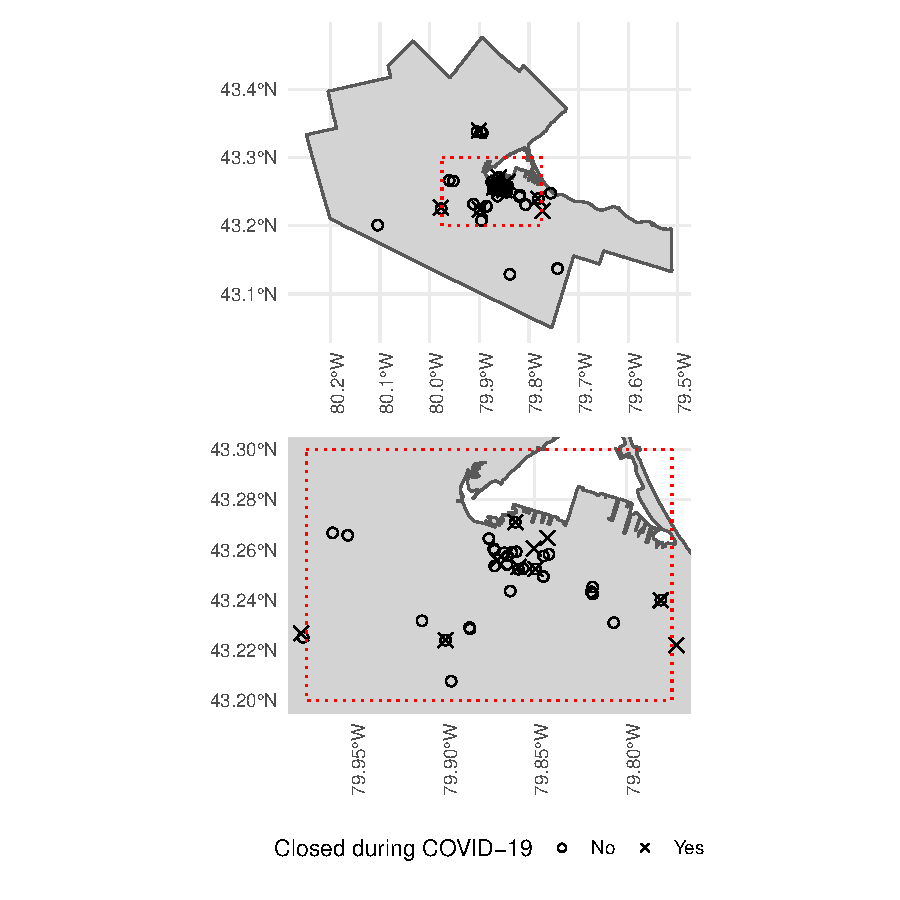
\includegraphics[width=1\linewidth]{Accessibility-Foodbanks-Hamilton_files/figure-latex/plot-location-foodbanks-1} \caption{\label{fig:foodbanks}Location of food banks/services and operation status; the dotted box is an inset of the central part of the City of Hamilton}\label{fig:plot-location-foodbanks}
\end{figure}

\begin{figure}
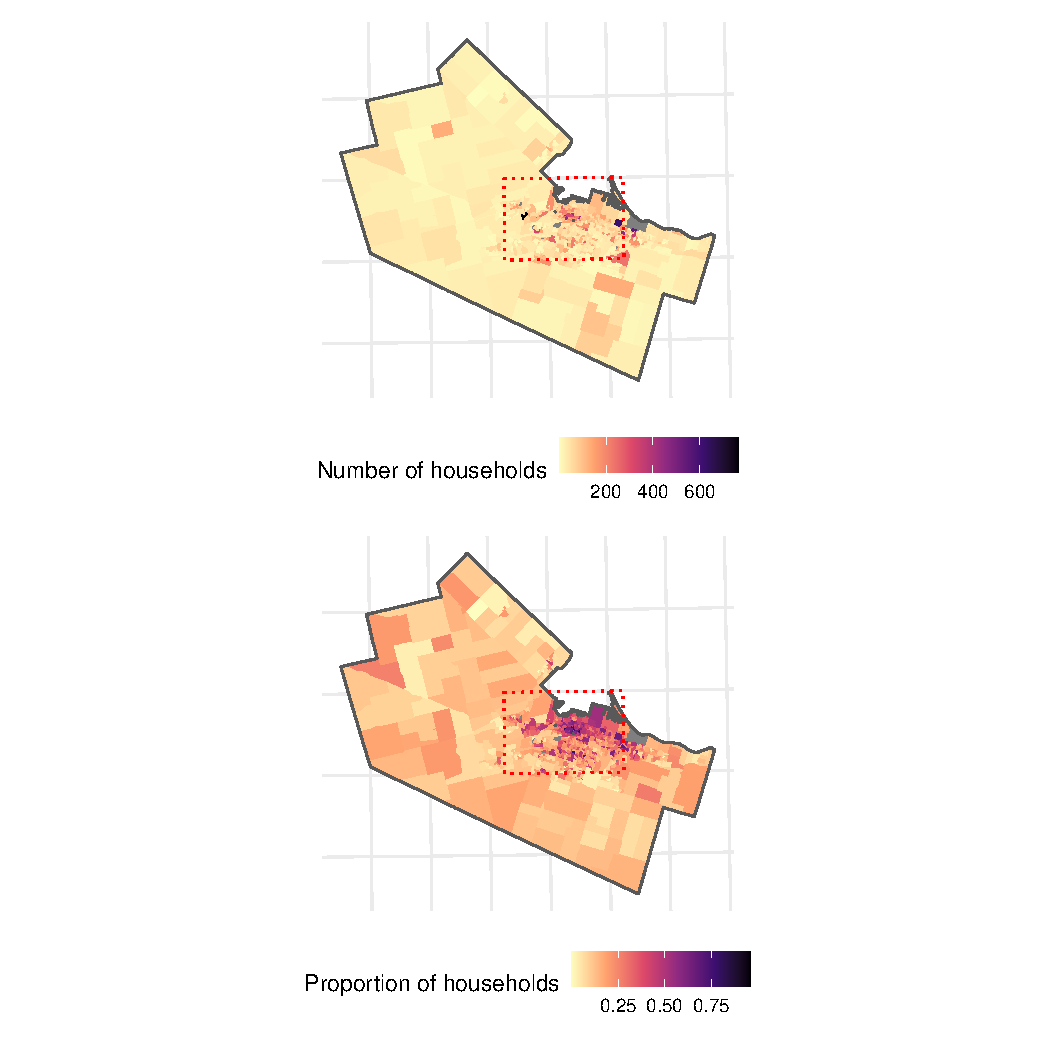
\includegraphics[width=1\linewidth]{Accessibility-Foodbanks-Hamilton_files/figure-latex/plot-low-income-households-1} \caption{\label{fig:low-income-households}Number and proportion of households with incomes less than CAD40,000.}\label{fig:plot-low-income-households}
\end{figure}

To implement the accessibility calculations, we must select a
distance-decay function. In this task we find limited support in the
literature, which is mostly silent on the travel patterns of people who
visit food banks and community food services. For this reason, we opt
for a simple cumulative opportunities function as follows:

\[
w_{ij}=
\begin{cases}
1 & \text{ if } ett_{ij}\le \delta\\
0 & \text{ otherwise}
\end{cases}
\]

\noindent where \(ett_{ij}\) is the multimodal expected travel time as
described previously, and \(\delta\) is a travel threshold. When the
expected travel time exceeds this threshold, a facility is no longer
considered accessible. Moreover, the weights are standardized for the
balanced floating catchment area approach.

Figure \ref{fig:sensitivity-analysis} shows the results of conducting a
sensitivity analysis of the system-wide accessibility as we vary the
threshold (considering the situation before the pandemic). There is a
clear pattern whereby more strict values of \(\delta\) are associated
with higher levels of system-wide accessibility: while increases in
accessibility that result from decreases in the travel time window might
seem counter-intuitive, this is a result of lower \emph{congestion},
since fewer households are serviced and thus competition for the same
resources is more limited. System-wide accessibility declines with
higher values of \(\delta\): as more households are serviced, congestion
grows and the level of service declines, although this happens at a
declining rate. We are not aware of any research that explains how long
people are expected to travel for food banks, but we note that in
developing countries, accessible sources of drinking water are those
that can be reached in less than 30 minutes (round trip, see UNICEF-WHO,
2019). There is no reason why people in affluent countries should be
expected to spend more time travelling for a basic necessity such as
food. Accordingly, we adopt a 15-minute threshold for the analysis
(representing a one-way trip). This threshold is also approximately
where the rate of change in accessibility slows down.

\begin{figure}
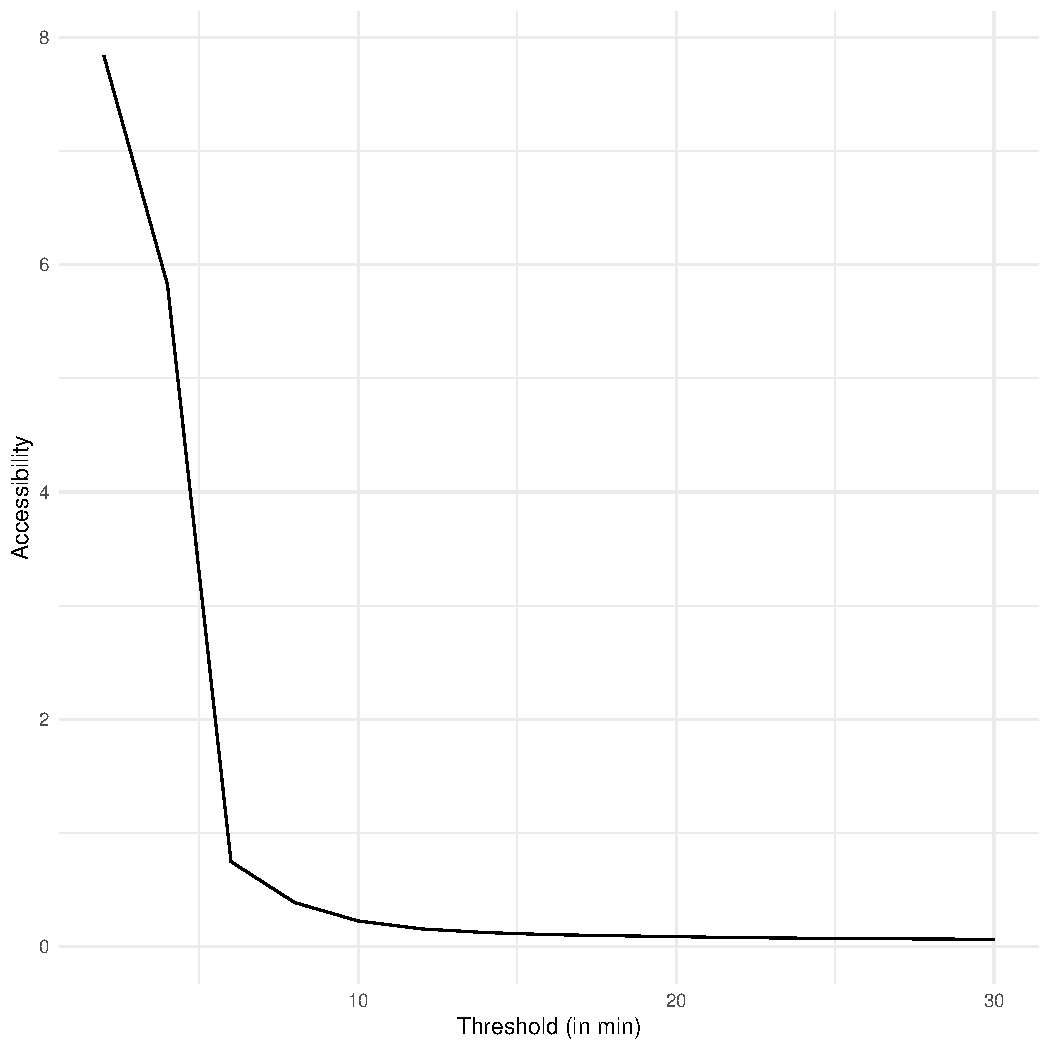
\includegraphics[width=0.6\linewidth]{Accessibility-Foodbanks-Hamilton_files/figure-latex/plot-results-sensitivity-analysis-1} \caption{\label{fig:sensitivity-analysis}Accessibility as a function of threshold}\label{fig:plot-results-sensitivity-analysis}
\end{figure}

Using the 15-minute threshold, we find that the system-wide
accessibility was 0.078 (food banks/service locations per low income
household in the city) before COVID-19, but declined to 0.048 during the
pandemic. It is striking that although almost 76\% of facilities
remained in operation during the pandemic, there was a loss of
accessibility greater than 39\%, suggesting the location of emergency
and community food services plays an important role in serving those in
need.

Turning to the location of individual facilities, the levels of service
offered before and during the pandemic are shown in Figure
\ref{fig:levels-of-service}. The level of service is functionally the
inverse of the number of low-income households in the travel-mode
weighted travel time catchment area of the facilities (this is because
\(S_j=1 \forall j\), i.e., each location represents a ``capacity'' of
1). Higher values mean that a facility is expected to service fewer
households. Conversely, lower values indicate greater congestion.

The general pattern of the levels of service is similar before and
during the pandemic, with lower values in the center of the city where
low-income households exhibit multimodal trip patterns that favour
proximate service locations. Three more peripheral facilities towards
the south of the city have moderate levels of service, presumably
because they are expected to service relatively suburban/exurban
populations generally reliant on automobiles for travel. During the
pandemic, however, the levels of service dropped, in some cases quite
substantially. The pattern of the losses in level of service, moreover,
is not uniform. The upper pane of Figure
\ref{fig:levels-of-service-changes} shows that the peripheral facilities
in the suburban/exurban parts of the city saw major declines during the
pandemic as more urban locations closed and demand increased for the
remaining locations. Further, the inset map shows that the levels of
service also deteriorated in the central part of the city. However, the
loss of level of service was not as large in the core (where most of the
food banks/services are found), but instead was more marked in the inner
ring around the core, where facilities may have faced greater demand
from both central city and suburban populations after the closure of
service locations during the pandemic.

\begin{figure}
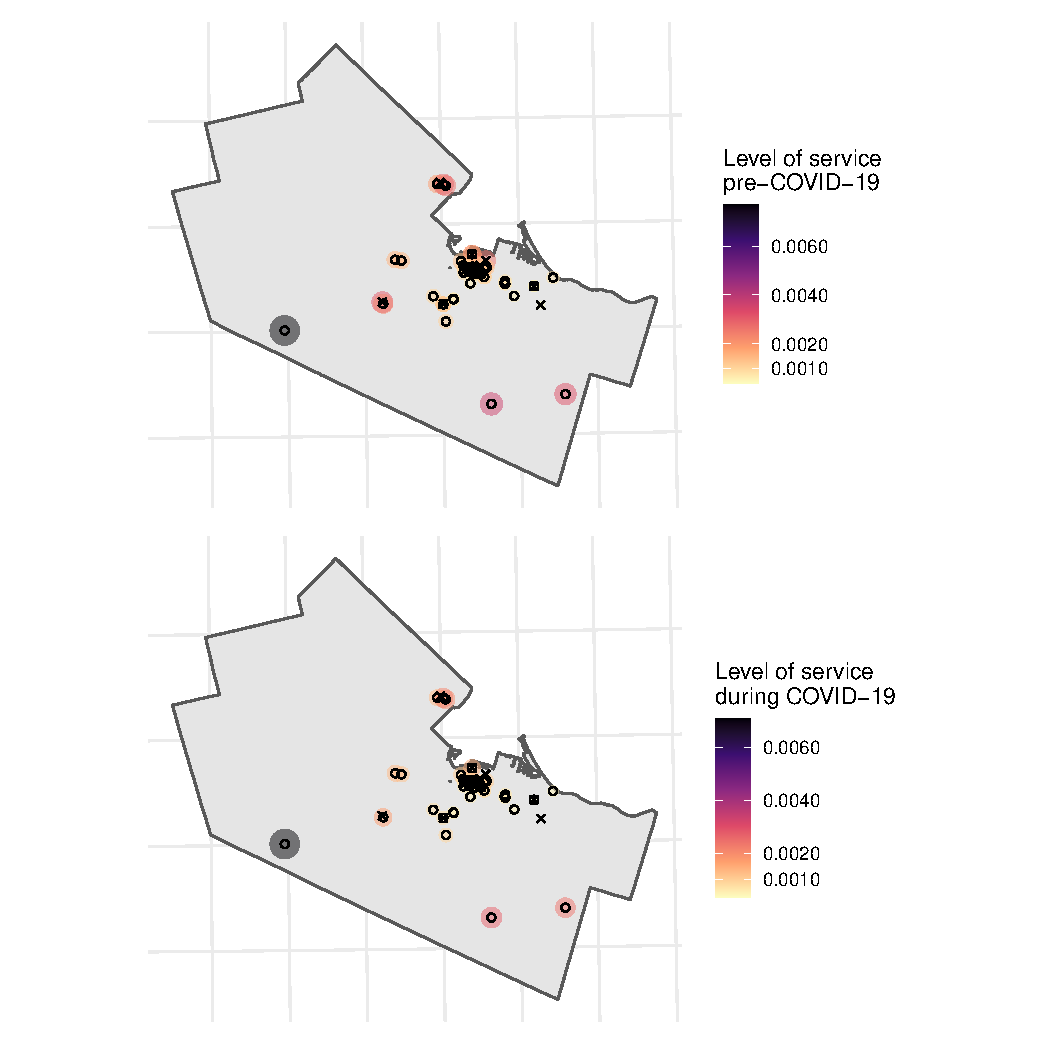
\includegraphics[width=1\linewidth]{Accessibility-Foodbanks-Hamilton_files/figure-latex/plot-levels-of-service-1} \caption{\label{fig:levels-of-service}Levels of service at each facility pre-COVID-19 (top panel) and during COVID-19 (bottom panel).}\label{fig:plot-levels-of-service}
\end{figure}

\begin{figure}
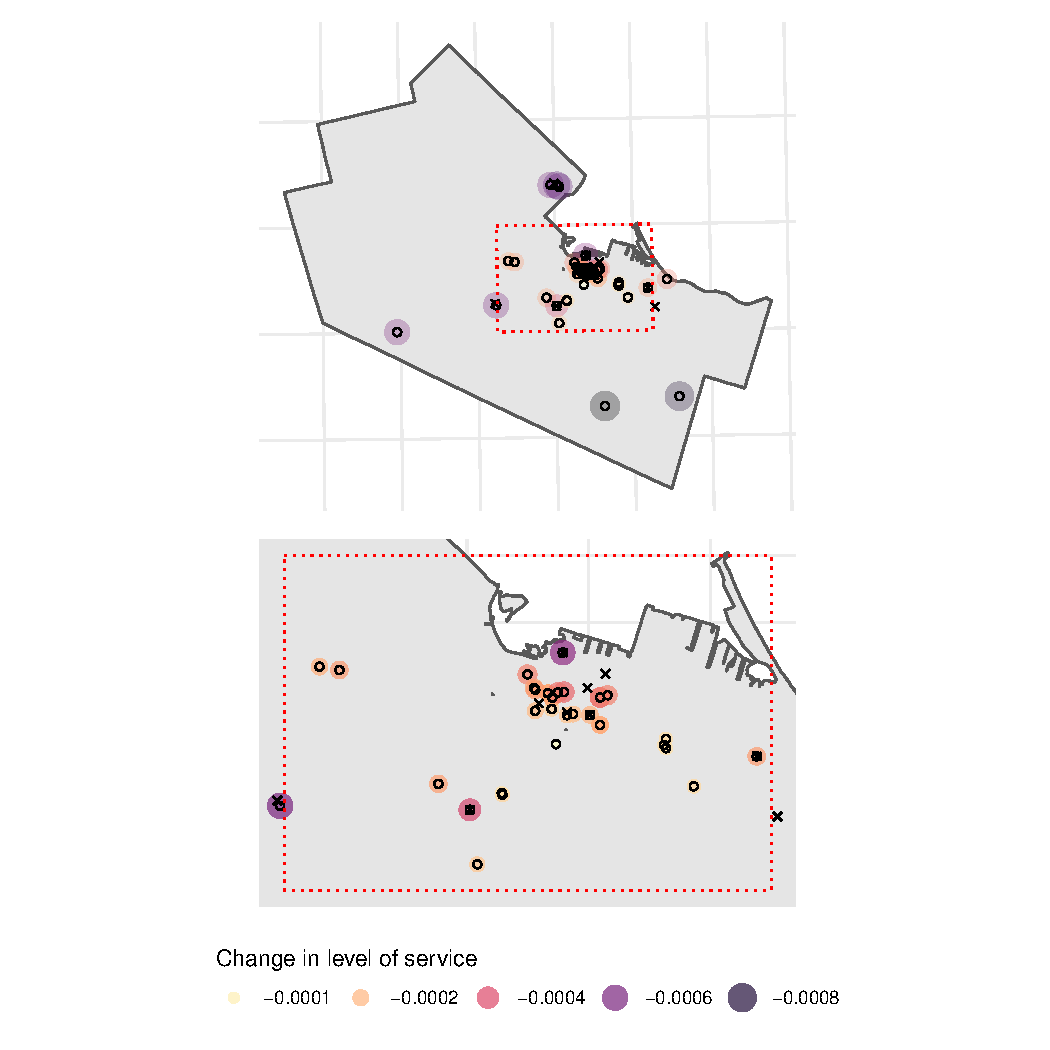
\includegraphics[width=1\linewidth]{Accessibility-Foodbanks-Hamilton_files/figure-latex/plot-levels-of-service-changes-1} \caption{\label{fig:levels-of-service-changes}Changes in levels of service at each facility from pre-COVID-19 to during COVID-19.}\label{fig:plot-levels-of-service-changes}
\end{figure}

To further elucidate this issue, we now turn to the results of the
accessibility analysis. As with the level of service of individual
facilities, the general pattern of accessibility before and during the
pandemic is similar. Figure \ref{fig:accessibility} reveals that,
compared with the outer rural zones, the more urban zones of the city
generally exhibit higher accessibility to food banks and food service
locations. However, the pattern is not particularly smooth - this is
largely attributable to the weighting of travel times by mode of
transportation according to the trip patterns of low-income household
respondents captured by the TTS. For example, in zones where low-income
households make a high proportion of trips by walking, access to food
bank locations by walking is afforded a concomitantly high weight in our
calculations of travel time compared to transit or car travel. From
this, highly-accessible locations result from a mix of characteristics:
low-income households in locations where travel options that align with
zonal modal split are available to connect them to food bank locations
with high levels of service within 15 minutes. This seems to track with
the experience of some users of these services, as reported by
Smith-Carrier et al. (2017).

\begin{figure}

{\centering 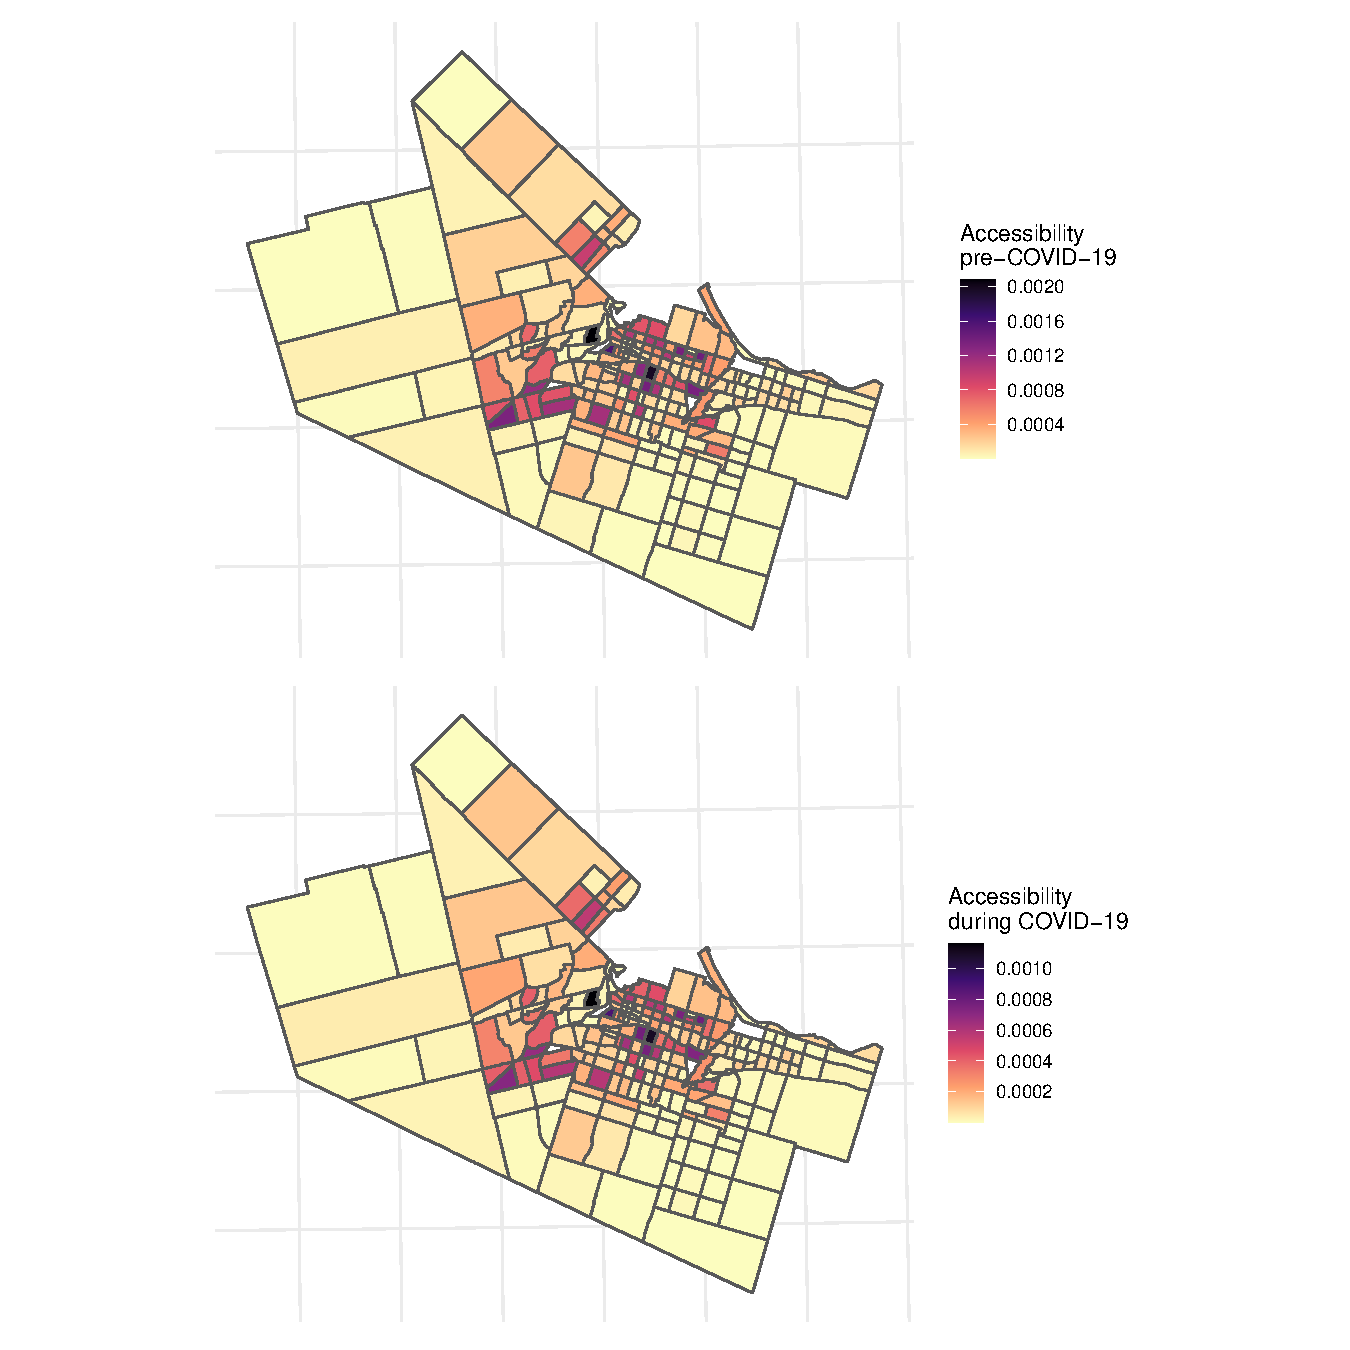
\includegraphics[width=1\linewidth]{Accessibility-Foodbanks-Hamilton_files/figure-latex/plot-accessibility-1} 

}

\caption{\label{fig:accessibility}Accessibility by traffic analysis zone pre-COVID-19 (top panel) and during COVID-19 (bottom panel).}\label{fig:plot-accessibility}
\end{figure}

We find that the accessibility landscape deteriorated substantially
during the pandemic, with accessibility dropping on average by almost
38\%, but with large variations: some zones experienced changes in
accessibility of only about 8\%, whereas the most affected zone saw a
loss of accessibility of almost 96\%. Figure
\ref{fig:accessibility-changes-with-local-i} shows the changes in
accessibility. Every zone is worse off after the closure of facilities
during the pandemic, but some parts of the city seem to have been
particularly affected. To better highlight these changes, we used a
local indicator of spatial autocorrelation (Anselin, 1995) to explore
the pattern of change in accessibility. Twenty-four TAZs are flagged as
having significantly large losses of accessibility (at \(p\le 0.10\),
without correcting for multiple comparisons). Those zones are
highlighted in the figure, where it can be seen that they form more or
less compact neighborhoods. Remarkably, the largest significant drops in
accessibility are not downtown, but located in two cases in the
industrial north of the city, in one case in an inner suburb above the
escarpment, and lastly in a more suburban/exurban region in the
south-west.

\begin{figure}

{\centering 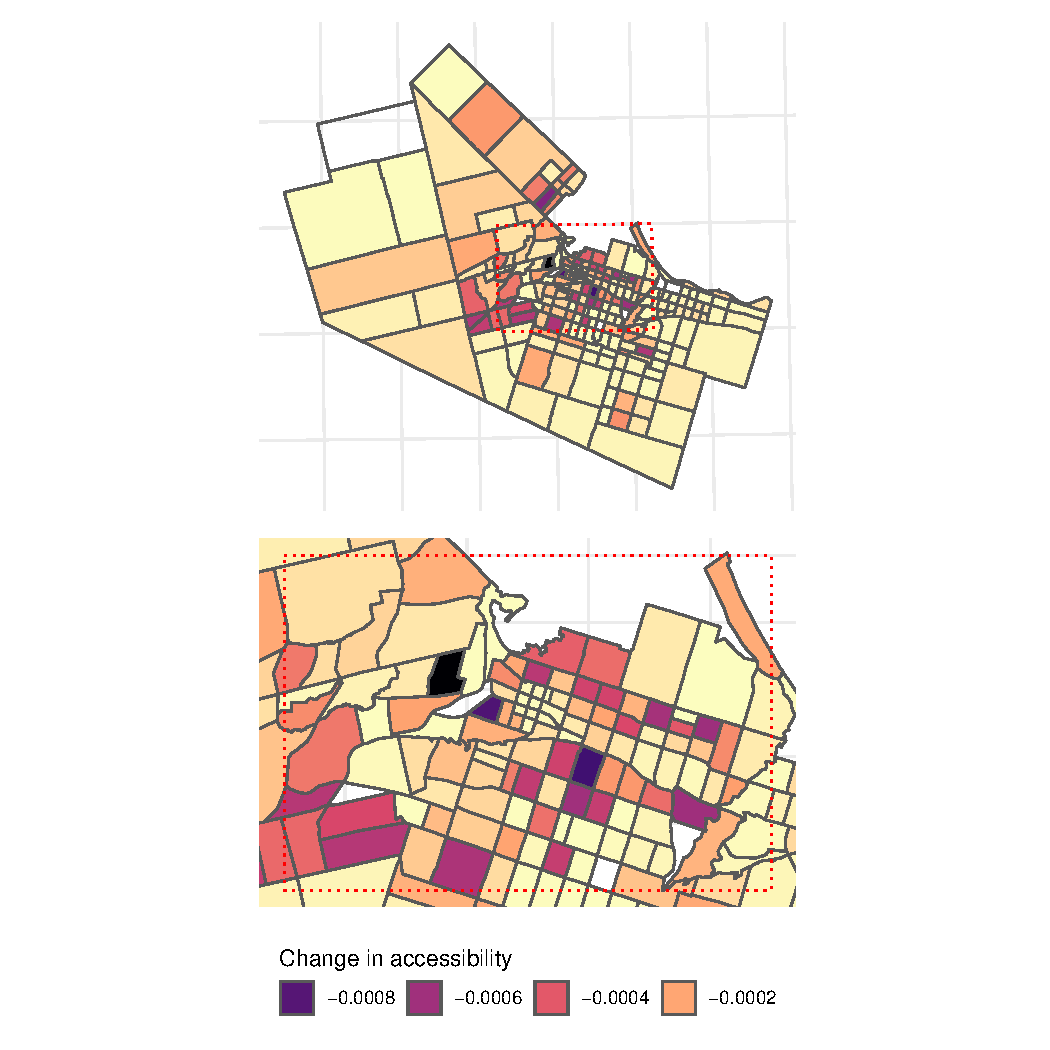
\includegraphics[width=1\linewidth]{Accessibility-Foodbanks-Hamilton_files/figure-latex/plot-accessibility-changes-1} 

}

\caption{\label{fig:accessibility-changes}Changes in accessibility from pre-COVID-19 to during COVID-19.}\label{fig:plot-accessibility-changes}
\end{figure}

\begin{figure}
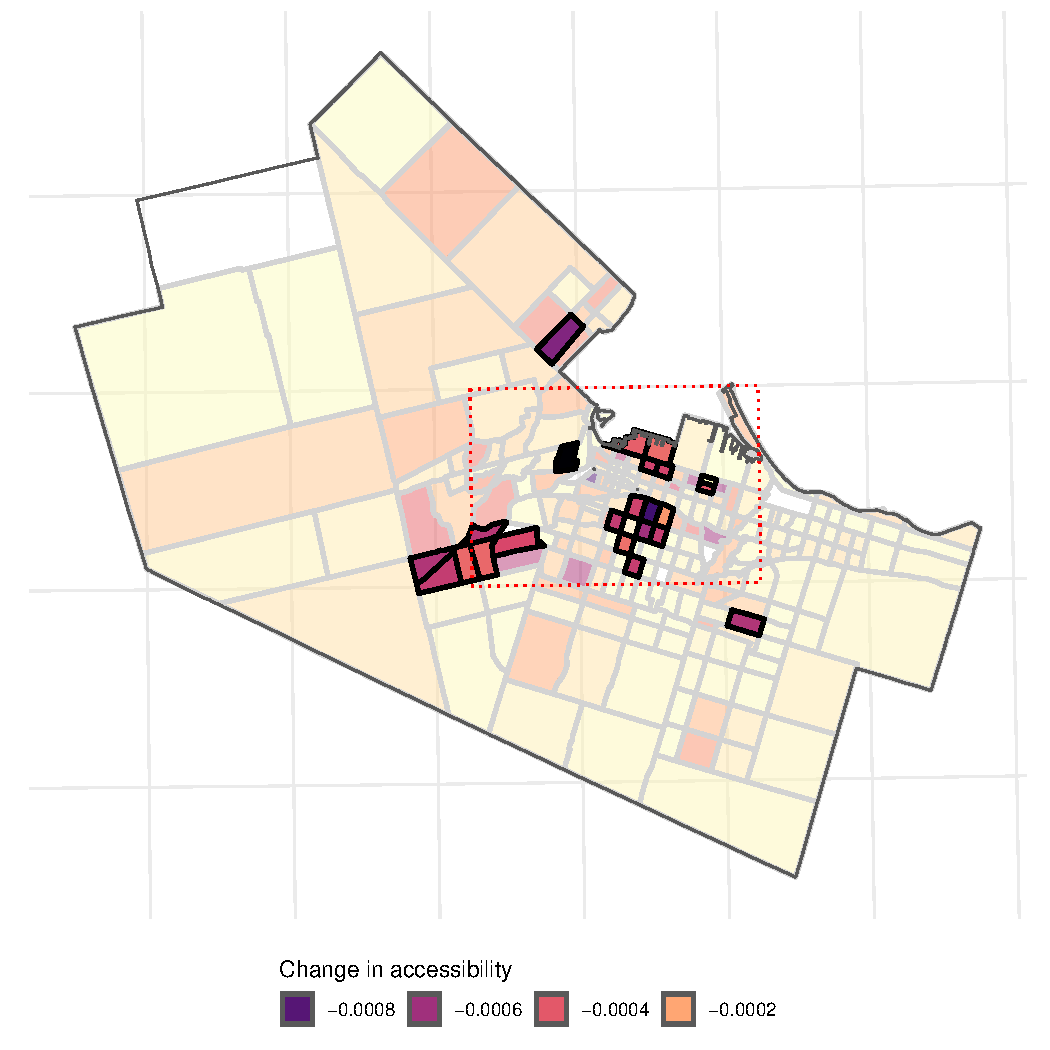
\includegraphics[width=1\linewidth]{Accessibility-Foodbanks-Hamilton_files/figure-latex/plot-local-i-1} \caption{\label{fig:accessibility-changes-with-local-i}Changes in accessibility from pre-COVID-19 to during COVID-19. Highlighted areas had significantly large changes in accessibility according to Local Moran's I.}\label{fig:plot-local-i}
\end{figure}

For the more suburban clusters of zones, the decrease in accessibility
is derived from the closure of locations throughout the city reachable
by car. In the cluster of central suburban zones for example, low-income
households in the outer ring of zones that exhibit medium to high
decreases in accessibility within this cluster appear to be largely
auto-dependent in their tripmaking, which each each exhibiting between
85-100\% of their modal split for car trips. This results in the parcels
within these zones having a large number of potentially accessible
locations in the travel time matrix. But by extension, the change in
accessibility over the pre- and during-COVID-19 time periods is affected
not only by the closure of service locations proximate to the zones, but
also the locations in the central city. The zone with the greatest
decrease in accessibility within this cluster (-0.0009) has a high rate
of car trips and connects to the most facility locations in total as
well as those that stayed open or closed.

In the cluster to the south-west, the decrease in accessibility is
predominately driven by the closure of a high level-of-service Community
Meals provider. However, like the more central suburban zones,
low-income households within this cluster are also between 90\% to 100\%
auto-dependent in their trip-making in the TTS. The story is similar for
the zone located in the north-west that exhibits the greatest decrease
in accessibility. Here, low-income households responding to the TTS
conducted 100\% of their trips by car and, as a result, dwellings within
this zone have access to the second-highest number of food bank and
service locations within 15 minutes. However, this also means zonal
accessibilities are greatly affected by the number of closures
throughout the city. Finally, in the city's north end and north-east
zones, low-income households exhibit a mixture of tripmaking behaviour
in the TTS. Households in some zones take transit more often and one
zone in particular has 100\% of its trips by walking. For these zones,
the decrease in accessibility tends to be a product of the closure of
several inner-city food bank and service locations reachable by multiple
modes.

Just as the effects of the closures appear to have been uneven in space,
they also seem to have had different impacts on various population
segments. Using data on low income individuals by age drawn from the
TTS, Table \ref{tab:accessibility-by-age} shows the estimated number of
people in each age group by their level of accessibility before and
during the pandemic. Here, it is important to note that the quartiles
are relative: people in the top 25\% of accessibility still have lower
accessibility during the pandemic than before. In reality, every
population group is worse off during the pandemic in terms of their
accessibility to food banks and services in the City of Hamilton.
However, some age groups were affected more. As seen in the table, the
distribution within quartiles for adults changed only slightly, and in
fact there are fewer adults in the bottom three quartiles as some found
themselves in the (deteriorated) top quartile of accessibility during
the pandemic. The story is different for seniors, a greater number of
whom are now in the third quartile, due to a combination of seniors
facing a worse accessibility situation, and just a few moving from the
bottom quartile (pre-pandemic) to the third during the pandemic. Those
aged 18 and less appear to have fared worse, and the largest change is
in the number of children who were in the third quartile before the
pandemic and found themselves in the bottom accessibility class during
the pandemic. In fact, when we compare the total population serviced
before and during the pandemic, we see that a large number of children,
adults, and seniors were no longer in the catchment areas of service
locations (last row of Table \ref{tab:accessibility-by-age}). It is
remarkable that despite the loss of population serviced, accessibility
still declined for those still within the catchment regions of these
services.

These results suggest that, through a combination of the typical modes
of transportation of lower income households and the spatial
distribution of the population, the food bank/service locations closed
had a differential impact that more greatly affected the youngest among
the population in low income households.

\begin{table}[!h]

\caption{\label{tab:table-accessibility-by-age-group}\label{tab:accessibility-by-age}Population at each accessibility level by age group among members households with incomes less than CAD40,000.}
\centering
\resizebox{\linewidth}{!}{
\begin{tabular}[t]{lcccccc}
\toprule
\multicolumn{1}{c}{ } & \multicolumn{3}{c}{Pre-COVID-19} & \multicolumn{3}{c}{During COVID-19} \\
\cmidrule(l{3pt}r{3pt}){2-4} \cmidrule(l{3pt}r{3pt}){5-7}
Accessibility Quartile & Children (age $\le$ 18) & Adults (19-64) & Seniors (age $\ge$ 65) & Children (age $\le$ 18) & Adults (19-64) & Seniors (age $\ge$ 65)\\
\midrule
\cellcolor{gray!6}{Top 25\%} & \cellcolor{gray!6}{2,048} & \cellcolor{gray!6}{7,031} & \cellcolor{gray!6}{3,632} & \cellcolor{gray!6}{1,956 (-4.49\%)} & \cellcolor{gray!6}{6,138 (-12.7\%)} & \cellcolor{gray!6}{3,338 (-8.09\%)}\\
Second 25\% & 2,190 & 9,631 & 5,023 & 2,365 (7.99\%) & 10,833 (12.48\%) & 5,400 (7.51\%)\\
\cellcolor{gray!6}{Third 25\%} & \cellcolor{gray!6}{3,239} & \cellcolor{gray!6}{12,694} & \cellcolor{gray!6}{6,875} & \cellcolor{gray!6}{3,082 (-4.85\%)} & \cellcolor{gray!6}{12,612 (-0.65\%)} & \cellcolor{gray!6}{7,064 (2.75\%)}\\
Bottom 25\% & 3,711 & 13,220 & 7,648 & 3,038 (-18.14\%) & 11,811 (-10.66\%) & 6,308 (-17.52\%)\\
\midrule
\cellcolor{gray!6}{Total population} & \cellcolor{gray!6}{11,189} & \cellcolor{gray!6}{42,576} & \cellcolor{gray!6}{23,178} & \cellcolor{gray!6}{10,441 (-6.69\%)} & \cellcolor{gray!6}{41,395 (-2.77\%)} & \cellcolor{gray!6}{22,110 (-4.61\%)}\\
\bottomrule
\multicolumn{7}{l}{\rule{0pt}{1em}\textit{Note: }}\\
\multicolumn{7}{l}{\rule{0pt}{1em}Population values have been rounded.}\\
\multicolumn{7}{l}{\rule{0pt}{1em}The values in brackets for population during COVID-19 are the changes from before the pandemic.}\\
\end{tabular}}
\end{table}

\hypertarget{conclusions}{%
\section{Conclusions}\label{conclusions}}

Food insecurity is a significant issue for many Canadian households and
while emergency and community food services can provide some relief, the
COVID-19 pandemic has in all probability increased food insecurity for
many households. To compound matters, the pandemic has also resulted in
major disruptions, including to employment, mobility alternatives, and
to emergency and community food services. In response, this research has
sought to better understand accessibility to food banks and food service
locations, as well as how the closure of some locations over the pre-
and during-COVID time periods affected the potential for low-income
households to reach these amenities.

Previous work has noted the important role of geography alongside other
socio-economic and demographic indicators in household access to healthy
food. The present papers is, to the best of our knowledge, among the
first studies to focus on the geographic component of accessibility to
emergency food services (Allen and Farber, 2021). Using the balanced
floating catchment area method to account for population demand and
congestion effects at service points, we estimated multi-modal
accessibility to emergency and community food service locations for
low-income households. The weighting of travel time estimates by the
modal split in different zonal geographies tailors the results to
patterns of travel behaviour captured in the regional travel survey.
Moreover, our parcel-level analysis presents a disaggregate approach to
estimating accessibility based on the locations of residential parcels
and dwellings. Beyond accounting for the inflation of demand that occurs
in traditional floating catchment area methods, our application of the
balanced floating catchment area approach offers a novel analysis of
accessibility to emergency and community food services that is sensitive
to the locations of low-income households, information on their age
distributions and typical trip-making behaviour, the locations of
services, their operations over time, and the characteristics of the
city's multi-modal transportation network.

Our results show that while accessibility levels were lower in the
city's more car-oriented suburban and rural areas to begin with, the
closure of 14\% of the city's emergency and community food service
locations during the pandemic resulted in an overall decrease in
accessibility across the city. However, these effects were not uniform
over space or for different population groups. Since the balanced
floating catchment area method takes into account changes in demand and
congestion for service providers, the closure of some services
reverberates throughout the catchment areas of the whole city. For some
suburban zones, the closure of a relatively high level-of-service
location results in the remaining services being spread over a larger
population. In others, high auto dependence for trips leads to decreases
in accessibility that accumulate due to the loss of several locations
initially reachable within 15 minutes by car. Reductions in
accessibility in the city's more urban north end, where low-income
households conduct higher proportions of trips by transit and walking,
emphasize the importance of geographic proximity in the potential to
reach service locations for these residents. Beyond geography, the
results also highlight the differential impact of closures during
COVID-19 on population groups, with seniors and children being the two
most impacted groups.

It is important to note that the degree to which our low-income cut-off
of CAD\$40,000 reflects food insecurity in the different zones of the
study area is not known. We also consider all emergency and community
food service locations equally. Information on differential capacities
at food provider locations is currently not collected, and given the
closure of facilities was not possible to obtain. Data on services, such
as the number of meals served, could be used to refine the analysis in
the future. Moreover, while the travel survey allows us to model
multi-modal accessibilities that align with travel behaviour observed in
the travel survey and capture differences in accessibility by age
categories, the use of travel survey data for modelling food insecurity
also has its limitations. Research into the population weighting methods
used in the TTS note that the survey may under-count the lowest- and
highest-income households in the survey study region, although the
magnitude of this under-counting is unknown, and approximately 20\% of
respondents to the 2016 survey did not report their income (Rose, 2018).
In that regard, the modal splits of low-income households observed
through the TTS data may not accurately reflect the travel behaviours of
food insecure populations, and our estimates might in fact be somewhat
conservative if those households who do not report income rely more on
walking and/or transit for their mobility needs.

In the absence of information regarding how food insecure households
travel to food banks and related services, we examined accessibility to
food banks using a 15 minutes (one-way) travel time threshold. The fact
that we must rely on a standard created for accessible drinking water in
the developing world only serves to highlight the tragedy of food
insecurity in an affluent country like Canada. More broadly, it points
to the absurd need to understand how a bad situation was made worse by
the pandemic: in effect, the analysis reveals that disparities in the
need for emergency and community food services predated the pandemic,
that the pandemic contributed to the deterioration of these services,
and that populations already in distress, particularly children, ended
up in an even more adverse state. How much worse, it is impossible to
say, mainly because there is also a dearth of information, let alone
standards, regarding \emph{acceptable} or \emph{sufficient} level of
service when it comes to emergency food services.

While on the one hand this work suggests that inequities in the
accessibility to emergency and community food services could be improved
through accessibility standards that promote changes in the geographic
distribution of service locations and transportation network
characteristics, in fact, we would argue that the standard should be
that no household faced food insecurity. As others have noted (Men and
Tarasuk, 2021; e.g., Poppendieck, 1999) the root of food insecurity is
income poverty and unless it is eliminated, there will continue to be a
place for emergency food and community food services. In addition to
providing food, these services satisfy social needs by offering a social
setting for seniors or by helping to connect households in need with
longer term supports. From a food security perspective, on the other
hand, these services should work only as a short term solution, and not
as a semi-permanent feature of life for some of our fellow human beings.
From a human rights perspective, long-term reliance on emergency food
services should be as unacceptable in Canada as lack of clean drinking
water within 30 minutes is elsewhere. Thus, while our analysis is
valuable to map the suffering caused by food insecurity, from a policy
perspective, maintaining a robust social safety net that includes
Employment Insurance and paid sick days are better tools to reduce this
suffering than increasing the accessibility of emergency food services
for food insecure populations.

\hypertarget{references}{%
\section*{References}\label{references}}
\addcontentsline{toc}{section}{References}

\hypertarget{refs}{}
\begin{CSLReferences}{1}{0}
\leavevmode\hypertarget{ref-foodpolicy2019}{}%
Agriculture, Canada, A.-F., 2019. Food policy for canada. Government of
Canada.

\leavevmode\hypertarget{ref-allen2021Changes}{}%
Allen, J., Farber, S., 2021. Changes in transit accessibility to food
banks in toronto during COVID-19. Findings.
doi:\href{https://doi.org/10.32866/001c.24072}{10.32866/001c.24072}

\leavevmode\hypertarget{ref-anselin1995local}{}%
Anselin, L., 1995. Local indicators of spatial association - LISA.
Geographical Analysis 27, 93--115.

\leavevmode\hypertarget{ref-arribas2021open}{}%
Arribas-Bel, D., Green, M., Rowe, F., Singleton, A., 2021. Open data
products: A framework for creating valuable analysis-ready data. Journal
of Geographical Systems.
doi:\href{https://doi.org/10.1007/s10109-021-00361-7}{10.1007/s10109-021-00361-7}

\leavevmode\hypertarget{ref-bazerghi2016role}{}%
Bazerghi, C., McKay, F.H., Dunn, M., 2016. The role of food banks in
addressing food insecurity: A systematic review. Journal of community
health 41, 732--740.

\leavevmode\hypertarget{ref-behan2008smart}{}%
Behan, K., Maoh, H., Kanaroglou, P., 2008. Smart growth strategies,
transportation and urban sprawl: Simulated futures for hamilton,
ontario. The Canadian Geographer/Le G{é}ographe canadien 52, 291--308.
doi:\url{https://doi.org/10.1111/j.1541-0064.2008.00214.x}

\leavevmode\hypertarget{ref-bhattacharya2004poverty}{}%
Bhattacharya, J., Currie, J., Haider, S., 2004. Poverty, food
insecurity, and nutritional outcomes in children and adults. Journal of
health economics 23, 839--862.
doi:\url{https://doi.org/10.1016/j.jhealeco.2003.12.008}

\leavevmode\hypertarget{ref-black2020examining}{}%
Black, J.L., Seto, D., 2020. Examining patterns of food bank use over
twenty-five years in vancouver, canada. VOLUNTAS: International Journal
of Voluntary and Nonprofit Organizations 31, 853--869.
doi:\url{https://doi.org/10.1007/s11266-018-0039-2}

\leavevmode\hypertarget{ref-boucher2017ontario}{}%
Boucher, B.A., Manafò, E., Boddy, M.R., Roblin, L., Truscott, R., 2017.
The ontario food and nutrition strategy: Identifying indicators of food
access and food literacy for early monitoring of the food environment.
Health promotion and chronic disease prevention in Canada : research,
policy and practice 37, 313--319.
doi:\href{https://doi.org/10.24095/hpcdp.37.9.06}{10.24095/hpcdp.37.9.06}

\leavevmode\hypertarget{ref-brunsdon2020opening}{}%
Brunsdon, C., Comber, A., 2020. Opening practice: Supporting
reproducibility and critical spatial data science. Journal of
Geographical Systems 1--20.
doi:\href{https://doi.org/10.1007/s10109-020-00334-2}{10.1007/s10109-020-00334-2}

\leavevmode\hypertarget{ref-dbfb2020}{}%
DBFB, 2020. Who's hungry 2020. Daily Bread Food Bank.

\leavevmode\hypertarget{ref-delamater2013spatial}{}%
Delamater, P.L., 2013. Spatial accessibility in suboptimally configured
health care systems: A modified two-step floating catchment area
(M2SFCA) metric. Health \& Place 24, 30--43.
doi:\url{https://doi.org/10.1016/j.healthplace.2013.07.012}

\leavevmode\hypertarget{ref-deluca2012code}{}%
DeLuca, P.F., Buist, S., Johnston, N., 2012. The code red project:
Engaging communities in health system change in hamilton, canada. Social
Indicators Research 108, 317--327.
doi:\url{https://doi.org/10.1007/s11205-012-0068-y}

\leavevmode\hypertarget{ref-deweese2020tale}{}%
DeWeese, J., Hawa, L., Demyk, H., Davey, Z., Belikow, A., El-geneidy,
A., 2020. A tale of 40 cities: A preliminary analysis of equity impacts
of COVID-19 service adjustments across north america. Findings.
doi:\href{https://doi.org/10.32866/001c.13395}{10.32866/001c.13395}

\leavevmode\hypertarget{ref-elgar2021relative}{}%
Elgar, F.J., Pickett, W., Pförtner, T.-K., Gariépy, G., Gordon, D.,
Georgiades, K., Davison, C., Hammami, N., MacNeil, A.H., Da Silva, M.A.,
others, 2021. Relative food insecurity, mental health and wellbeing in
160 countries. Social Science \& Medicine 268, 113556.
doi:\url{https://doi.org/10.1016/j.socscimed.2020.113556}

\leavevmode\hypertarget{ref-enns2020experiences}{}%
Enns, A., Rizvi, A., Quinn, S., Kristjansson, E., 2020. Experiences of
food bank access and food insecurity in ottawa, canada. Journal of
Hunger \& Environmental Nutrition 15, 456--472.
doi:\url{https://doi.org/10.1080/19320248.2020.1761502}

\leavevmode\hypertarget{ref-fbc2018}{}%
FBC, 2018. HungerCount 2018. Food Banks Canada.

\leavevmode\hypertarget{ref-fbc2020}{}%
FBC, 2020. A snapshot of food banks in canada and the COVID-19 crisis.
Food Banks Canada.

\leavevmode\hypertarget{ref-feedontario2019}{}%
FO, 2019. Report: Hunger map. Feed Ontario.

\leavevmode\hypertarget{ref-ghorbanzadeh2021spatial}{}%
Ghorbanzadeh, M., Kim, K., Erman Ozguven, E., Horner, M.W., 2021.
Spatial accessibility assessment of COVID-19 patients to healthcare
facilities: A case study of florida. Travel Behaviour and Society 24,
95--101. doi:\url{https://doi.org/10.1016/j.tbs.2021.03.004}

\leavevmode\hypertarget{ref-gundersen2018food}{}%
Gundersen, C., Tarasuk, V., Cheng, J., De Oliveira, C., Kurdyak, P.,
2018. Food insecurity status and mortality among adults in ontario,
canada. PloS one 13, e0202642.

\leavevmode\hypertarget{ref-hcf2018}{}%
HCF, 2018. Vital signs: A reflection of hamilton. Hamilton Community
Foundation.

\leavevmode\hypertarget{ref-hfs2019}{}%
HFS, 2019. Hamilton hunger report 2019. Hamilton Food Share.

\leavevmode\hypertarget{ref-holmes2018nothing}{}%
Holmes, E., Black, J.L., Heckelman, A., Lear, S.A., Seto, D., Fowokan,
A., Wittman, H., 2018. {``Nothing is going to change three months from
now''}: A mixed methods characterization of food bank use in greater
vancouver. Social Science \& Medicine 200, 129--136.
doi:\url{https://doi.org/10.1016/j.socscimed.2018.01.029}

\leavevmode\hypertarget{ref-hpl2021}{}%
HPL, 2021. Food access guide. Hamilton Public Library.

\leavevmode\hypertarget{ref-jakar2019turning}{}%
Jakar, G.S., Dunn, J.R., 2019. (Turning rust into gold?) Hamilton,
ontario and a canadian perspective of shrinking and declining cities.
Cities 94, 1--10. doi:\url{https://doi.org/10.1016/j.cities.2019.05.016}

\leavevmode\hypertarget{ref-jones2017food}{}%
Jones, A.D., 2017. Food insecurity and mental health status: A global
analysis of 149 countries. American journal of preventive medicine 53,
264--273. doi:\url{https://doi.org/10.1016/j.amepre.2017.04.008}

\leavevmode\hypertarget{ref-kirkpatrick2008food}{}%
Kirkpatrick, S.I., Tarasuk, V., 2008. Food insecurity is associated with
nutrient inadequacies among canadian adults and adolescents. The Journal
of nutrition 138, 604--612.
doi:\url{https://doi.org/10.1093/jn/138.7.1399}

\leavevmode\hypertarget{ref-laborde2020poverty}{}%
Laborde, D., Martin, W., Vos, R., 2020. Poverty and food insecurity
could grow dramatically as COVID-19 spreads. International Food Policy
Research Institute (IFPRI), Washington, DC.

\leavevmode\hypertarget{ref-latham2007determinants}{}%
Latham, J., Moffat, T., 2007. Determinants of variation in food cost and
availability in two socioeconomically contrasting neighbourhoods of
hamilton, ontario, canada. Health \& Place 13, 273--287.
doi:\url{https://doi.org/10.1016/j.healthplace.2006.01.006}

\leavevmode\hypertarget{ref-loopstra2012relationship}{}%
Loopstra, R., Tarasuk, V., 2012. The relationship between food banks and
household food insecurity among low-income toronto families. Canadian
Public Policy 38, 497--514.
doi:\href{https://doi.org/10.3138/cpp.38.4.497}{10.3138/cpp.38.4.497}

\leavevmode\hypertarget{ref-lovelace2021open}{}%
Lovelace, R., 2021. Open source tools for geographic analysis in
transport planning. Journal of Geographical Systems.
doi:\href{https://doi.org/10.1007/s10109-020-00342-2}{10.1007/s10109-020-00342-2}

\leavevmode\hypertarget{ref-luo2003measures}{}%
Luo, W., Wang, F.H., 2003. Measures of spatial accessibility to health
care in a GIS environment: Synthesis and a case study in the chicago
region. Environment and Planning B-Planning \& Design 30, 865--884.

\leavevmode\hypertarget{ref-mckay2021exploring}{}%
McKay, F.H., Bastian, A., Lindberg, R., 2021. Exploring the response of
the victorian emergency and community food sector to the COVID-19
pandemic. Journal of Hunger \& Environmental Nutrition 1--15.
doi:\href{https://doi.org/10.1080/19320248.2021.1900974}{10.1080/19320248.2021.1900974}

\leavevmode\hypertarget{ref-men2021food}{}%
Men, F., Tarasuk, V., 2021. Food insecurity amid the COVID-19 pandemic:
Food charity, government assistance and employment. Canadian Public
Policy COVID-19, e2021001.
doi:\href{https://doi.org/10.3138/cpp.2021-001}{10.3138/cpp.2021-001}

\leavevmode\hypertarget{ref-oemichen2016investigation}{}%
Oemichen, M., Smith, C., 2016. Investigation of the food choice,
promoters and barriers to food access issues, and food insecurity among
low-income, free-living minnesotan seniors. Journal of nutrition
education and behavior 48, 397--404.

\leavevmode\hypertarget{ref-olson1999nutrition}{}%
Olson, C.M., 1999. Nutrition and health outcomes associated with food
insecurity and hunger. The Journal of nutrition 129, 521S--524S.
doi:\url{https://doi.org/10.1093/jn/129.2.521S}

\leavevmode\hypertarget{ref-paez2019demand}{}%
Paez, A., Higgins, C.D., Vivona, S.F., 2019. Demand and level of service
inflation in floating catchment area (FCA) methods. PloS one 14,
e0218773.
doi:\href{https://doi.org/10.1371/journal.pone.0218773}{10.1371/journal.pone.0218773}

\leavevmode\hypertarget{ref-paez2010relative}{}%
Paez, A., Mercado, R.G., Farber, S., Morency, C., Roorda, M., 2010.
Relative accessibility deprivation indicators for urban settings:
Definitions and application to food deserts in montreal. Urban Studies
47, 1415--1438.
doi:\href{https://doi.org/10.1177/0042098009353626}{10.1177/0042098009353626}

\leavevmode\hypertarget{ref-paez2012measuring}{}%
Páez, A., Scott, D.M., Morency, C., 2012. Measuring accessibility:
Positive and normative implementations of various accessibility
indicators. Journal of Transport Geography 25, 141--153.
doi:\url{https://doi.org/10.1016/j.jtrangeo.2012.03.016}

\leavevmode\hypertarget{ref-pereira2021geographic}{}%
Pereira, R.H.M., Braga, C.K.V., Servo, L.M., Serra, B., Amaral, P.,
Gouveia, N., Paez, A., 2021a. Geographic access to COVID-19 healthcare
in brazil using a balanced float catchment area approach. Social Science
\& Medicine 273, 113773.
doi:\url{https://doi.org/10.1016/j.socscimed.2021.113773}

\leavevmode\hypertarget{ref-pereira2021r5r}{}%
Pereira, R.H.M., Saraiva, M., Herszenhut, D., Braga, C.K.V., Conway,
M.W., 2021b. r5r: Rapid realistic routing on multimodal transport
networks with r\textsuperscript{5} in r. Findings.
doi:\href{https://doi.org/10.32866/001c.21262}{10.32866/001c.21262}

\leavevmode\hypertarget{ref-poppendieck1999sweet}{}%
Poppendieck, J., 1999. Sweet charity?: Emergency food and the end of
entitlement. Penguin.

\leavevmode\hypertarget{ref-radke2000spatial}{}%
Radke, J., Mu, L., 2000. Spatial decomposition, modeling and mapping
service regions to predict access to social programs. Annals of
Geographic Information Sciences 6, 105--112.

\leavevmode\hypertarget{ref-ramsey2011food}{}%
Ramsey, R., Giskes, K., Turrell, G., Gallegos, D., 2011. Food insecurity
among australian children: Potential determinants, health and
developmental consequences. Journal of Child Health Care 15, 401--416.
doi:\url{https://doi.org/10.1177\%2F1367493511423854}

\leavevmode\hypertarget{ref-riches2002food}{}%
Riches, G., 2002. Food banks and food security: Welfare reform, human
rights and social policy. Lessons from canada? Social Policy \&
Administration 36, 648--663.

\leavevmode\hypertarget{ref-rose2018transportation}{}%
Rose, A., 2018. Transportation tomorrow survey 2016: Data expansion and
validation. Data Management Group, Department of Civil Engineering,
University of Toronty, Malatest \& Associates.

\leavevmode\hypertarget{ref-seligman2010food}{}%
Seligman, H.K., Laraia, B.A., Kushel, M.B., 2010. Food insecurity is
associated with chronic disease among low-income NHANES participants.
The Journal of nutrition 140, 304--310.

\leavevmode\hypertarget{ref-smith2017food}{}%
Smith-Carrier, T., Ross, K., Kirkham, J., Decker Pierce, B., 2017.
{`Food is a right\ldots{} nobody should be starving on our streets'}:
Perceptions of food bank usage in a mid-sized city in ontario, canada.
Journal of Human Rights Practice 9, 29--49.

\leavevmode\hypertarget{ref-statisticscanada2020food}{}%
Statistics Canada, 2020a. Food insecurity during the COVID-19 pandemic
(No. Catalogue no. 45280001).

\leavevmode\hypertarget{ref-statisticscanada2020licos}{}%
Statistics Canada, 2020b. Table 11-10-0241-01 low income cut-offs
(LICOs) before and after tax by community size and family size, in
current dollars. doi:\url{https://doi.org/10.25318/1110024101-eng}

\leavevmode\hypertarget{ref-stuff2004household}{}%
Stuff, J.E., Casey, P.H., Szeto, K.L., Gossett, J.M., Robbins, J.M.,
Simpson, P.M., Connell, C., Bogle, M.L., 2004. Household food insecurity
is associated with adult health status. The Journal of nutrition 134,
2330--2335.
doi:\href{https://doi.org/Oxford\%20University\%20Press}{Oxford University Press}

\leavevmode\hypertarget{ref-tarasuk2014food}{}%
Tarasuk, V., Dachner, N., Loopstra, R., 2014. Food banks, welfare, and
food insecurity in canada. British Food Journal.

\leavevmode\hypertarget{ref-tarasuk2020relationship}{}%
Tarasuk, V., Fafard St-Germain, A.-A., Loopstra, R., 2020. The
relationship between food banks and food insecurity: Insights from
canada. VOLUNTAS: International Journal of Voluntary and Nonprofit
Organizations 31, 841--852.
doi:\href{https://doi.org/10.1007/s11266-019-00092-w}{10.1007/s11266-019-00092-w}

\leavevmode\hypertarget{ref-tarasuk2019geographic}{}%
Tarasuk, V., Fafard St-Germain, A.-A., Mitchell, A., 2019. Geographic
and socio-demographic predictors of household food insecurity in canada,
2011--12. BMC Public Health 19, 12.
doi:\href{https://doi.org/10.1186/s12889-018-6344-2}{10.1186/s12889-018-6344-2}

\leavevmode\hypertarget{ref-tarasuk1999qualitative}{}%
Tarasuk, V., Reynolds, R., 1999. A qualitative study of community
kitchens as a response to income-related food insecurity. Canadian
Journal of Dietetic Practice and Research 60, 11.

\leavevmode\hypertarget{ref-tarasuk2009household}{}%
Tarasuk, V., Vogt, J., 2009. Household food insecurity in ontario.
Canadian Journal of Public Health 100, 184--188.
doi:\href{https://doi.org/10.1007/BF03405537}{10.1007/BF03405537}

\leavevmode\hypertarget{ref-topalovic2012light}{}%
Topalovic, P., Carter, J., Topalovic, M., Krantzberg, G., 2012. Light
rail transit in hamilton: Health, environmental and economic impact
analysis. Social Indicators Research 108, 329--350.
doi:\url{https://doi.org/10.1007/s11205-012-0069-x}

\leavevmode\hypertarget{ref-world2019progress}{}%
UNICEF-WHO, 2019. Progress on household drinking water, sanitation and
hygiene 2000--2017. Special focus on inequalities.

\leavevmode\hypertarget{ref-vanderlee2017food}{}%
Vanderlee, L., L'Abbé, M., 2017. Food for thought on food environments
in canada. Health promotion and chronic disease prevention in Canada :
research, policy and practice 37, 263--265.
doi:\href{https://doi.org/10.24095/hpcdp.37.9.01}{10.24095/hpcdp.37.9.01}

\leavevmode\hypertarget{ref-vonBergmann2021cancensus}{}%
von Bergmann, J., Shkolnik, D., Jacobs, A., 2021. Cancensus: R package
to access, retrieve, and work with canadian census data and geography.

\leavevmode\hypertarget{ref-wakefield2013sweet}{}%
Wakefield, S., Fleming, J., Klassen, C., Skinner, A., 2013. Sweet
charity, revisited: Organizational responses to food insecurity in
hamilton and toronto, canada. Critical Social Policy 33, 427--450.

\leavevmode\hypertarget{ref-wan2012three}{}%
Wan, N., Zou, B., Sternberg, T., 2012. A three-step floating catchment
area method for analyzing spatial access to health services.
International Journal of Geographical Information Science 26,
1073--1089.
doi:\href{https://doi.org/10.1080/13658816.2011.624987}{10.1080/13658816.2011.624987}

\leavevmode\hypertarget{ref-widener2018spatial}{}%
Widener, M.J., 2018. Spatial access to food: Retiring the food desert
metaphor. Physiology \& behavior 193, 257--260.
doi:\url{https://doi.org/10.1016/j.physbeh.2018.02.032}

\end{CSLReferences}


\end{document}
